\documentclass[portuguese]{sbc2025}%

\usepackage[misc,geometry]{ifsym}

\raggedbottom  % Prevent underfull vbox warnings

\usepackage{aas_macros}
\usepackage[bottom]{footmisc}

\usepackage{tabularray}
\usepackage{adjustbox}
\usepackage{stfloats}
\usepackage{placeins}
\usepackage{float}
\usepackage{tikz}
\usetikzlibrary{arrows.meta,positioning,fit,calc,matrix}

\usepackage{afterpage}
\usepackage{url}
\usepackage{pifont}

\setcitestyle{square}

\definecolor{engtitle}{rgb}{0.5,0.5,0.5}
\definecolor{orcidlogo}{rgb}{0.37,0.48,0.13}
\definecolor{unilogo}{rgb}{0.16, 0.26, 0.58}
\definecolor{maillogo}{rgb}{0.58, 0.16, 0.26}
\definecolor{darkblue}{rgb}{0.0,0.0,0.0}
\hypersetup{colorlinks,breaklinks,
            linkcolor=darkblue,urlcolor=darkblue,
            anchorcolor=darkblue,citecolor=darkblue}

\jyear{2025}

\category{Artigo de Pesquisa/Research Paper}
\title[Sistema de Monitoria-IC: Plataforma Web para Gestão de Monitorias Acadêmicas da UFBA]{Sistema de Monitoria-IC: Plataforma Web para Gestão Completa de Monitorias Acadêmicas da UFBA}
\engtitle{\textcolor{engtitle}{Sistema de Monitoria-IC: Web Platform for Complete Management of Academic Monitoring Programs at UFBA}}

\author[Sena et al. 2025]{
\affil{\textbf{Luis Felipe Cordeiro Sena}~\orcidlink{0009-0009-3997-3639}~\textcolor{blue}{\faEnvelopeO}~~[{Universidade Federal da Bahia}~|\href{mailto:luis.sena@ufba.br}{~{\textit{luis.sena@ufba.br}}}~]}

\affil{\textbf{Frederico Araújo Durão}~\orcidlink{0000-0002-7766-6666}~~[{Universidade Federal da Bahia}~| \href{mailto:fdurao@ufba.br}{{\textit{fdurao@ufba.br}}}~]}
}

\begin{document}

\begin{frontmatter}

\maketitle

\begin{mail}
Instituto de Computação, Universidade Federal da Bahia, Av. Milton Santos, s/n - Campus de Ondina, PAF 2, Salvador, BA, 40170-110, Brasil.
\end{mail}

\begin{abstract-pt}
A monitoria acadêmica é um processo fundamental nas universidades brasileiras que permite aos alunos desenvolverem habilidades pedagógicas enquanto auxiliam no processo de ensino-aprendizagem. Porém, o gerenciamento desse processo frequentemente enfrenta desafios relacionados à burocracia, falta de transparência e múltiplos processos manuais ineficientes. Este trabalho apresenta o desenvolvimento do Sistema de Monitoria-IC, uma plataforma web projetada para automatizar e simplificar todo o ciclo de vida dos projetos de monitoria na UFBA. A solução proposta digitaliza desde a criação de projetos pelos professores até a seleção de monitores, alocação de bolsas e geração de relatórios finais. O sistema foi desenvolvido utilizando tecnologias modernas como Next.js 15, TypeScript, tRPC, PostgreSQL e MinIO, seguindo princípios de engenharia de software que garantem escalabilidade e manutenibilidade. A arquitetura implementada separa claramente as responsabilidades entre um Sistema de Processamento de Transações (SPT) para operações cotidianas e funcionalidades gerenciais para análise e controle. A validação técnica através de testes end-to-end demonstra a robustez da solução. Os resultados esperados indicam que a automação proposta tende a eliminar retrabalho administrativo, aumentar a transparência por meio de histórico auditável e estabelecer uma base sólida para a modernização da gestão acadêmica na universidade.
\end{abstract-pt}

\begin{abstract-en}
Academic monitoring is a fundamental process in Brazilian universities that allows students to develop pedagogical skills while assisting in the teaching-learning process. However, managing this process often faces challenges related to bureaucracy, lack of transparency, and multiple inefficient manual procedures. This work presents the development of Sistema de Monitoria-IC, a web platform designed to automate and simplify the entire lifecycle of monitoring projects at UFBA. The proposed solution digitizes everything from project creation by professors to monitor selection, scholarship allocation, and final report generation. The system was developed using modern technologies such as Next.js 15, TypeScript, tRPC, PostgreSQL, and MinIO, following software engineering principles that ensure scalability and maintainability. The implemented architecture clearly separates responsibilities between a Transaction Processing System (TPS) for daily operations and managerial functionalities for analysis and control. Technical validation through end-to-end tests demonstrates the solution's robustness. Expected results indicate that the proposed automation tends to eliminate administrative rework, increase transparency through auditable history, and establish a solid foundation for modernizing academic management at the university.
\end{abstract-en}

\begin{pchaves}
Gestão Acadêmica, Sistema de Monitoria, Arquitetura de Software, Desenvolvimento Web, Automação de Processos.
\end{pchaves}

\begin{keywords}
Academic Management, Monitoring System, Software Architecture, Web Development, Process Automation.
\end{keywords}

\begin{dates}
% Informações serão preenchidas pelo editor antes da publicação
\end{dates}

\end{frontmatter}

\section{Introdução}
\label{sec:intro}

% Contextualização e Motivação (título removido conforme orientação; texto mantido)

A monitoria acadêmica representa um dos pilares fundamentais do ensino superior brasileiro, estabelecendo-se como uma prática pedagógica que beneficia simultaneamente monitores, estudantes e docentes. Regulamentada pela Lei nº 9.394/96 (Lei de Diretrizes e Bases da Educação Nacional), a monitoria permite que alunos com destacado desempenho acadêmico auxiliem seus pares no processo de aprendizagem, desenvolvendo competências didáticas enquanto aprofundam seus conhecimentos na disciplina \cite{Brasil1996}.

Na Universidade Federal da Bahia (UFBA), o programa de monitoria segue um fluxo complexo que envolve múltiplos atores e etapas interdependentes. O processo inicia-se com o planejamento semestral, quando a administração importa dados de disciplinas e professores. Em seguida, os docentes criam e submetem projetos de monitoria que precisam ser aprovados administrativamente. Após a aprovação, ocorre a publicação de editais internos, inscrição de candidatos, processo seletivo, alocação de bolsas, e finalmente, a consolidação de dados para envio à PROGRAD (Pró-Reitoria de Graduação).

A literatura de Sistemas de Informação fornece evidências de que a digitalização e a automação de processos reduzem custos transacionais, eliminam retrabalho e aumentam a confiabilidade e a auditabilidade dos registros \cite{Laudon_Laudon_2011, Davenport1993, Hammer1993}. Em contextos públicos e acadêmicos, iniciativas de governo digital e transformação digital têm sido associadas a ganhos de eficiência administrativa e transparência, desde que apoiadas por arquitetura tecnológica moderna e governança de dados adequada \cite{WorldBank2022, UNESCO2022}. No escopo deste trabalho, adotamos tais fundamentos para sustentar a proposta de um sistema unificado de monitoria, substituindo fluxos fragmentados por um \textit{workflow} padronizado, rastreável e escalável.

Apesar de sua importância reconhecida, a gestão dos programas de monitoria na UFBA ainda depende predominantemente de processos manuais e fragmentados. Formulários em papel, planilhas eletrônicas dispersas, comunicação via e-mail e ausência de um sistema centralizado caracterizam o cenário atual, resultando em ineficiências operacionais significativas. Essa realidade contrasta com a tendência global de digitalização e automação de processos administrativos no ambiente acadêmico, conforme defendem \cite{Laudon_Laudon_2011}, que argumentam que a tecnologia da informação constitui uma das principais ferramentas para alcançar excelência operacional.

\subsection{Identificação do Problema}

O processo de monitoria na UFBA é \textbf{lento}, \textbf{caro} e \textbf{opaco}. Do lado docente, há \textbf{retrabalho sistemático} (recriação de projetos a cada semestre), \textbf{dispersão de documentos} (planilhas, PDFs e e-mails) e \textbf{ausência de trilhas de auditoria} --- combinação que consome horas de atividades-fim e eleva o risco de erro. A seleção permanece \textbf{predominantemente manual} e \textbf{heterogênea} entre departamentos, impedindo comparabilidade de critérios e produzindo falhas de registro.

Para estudantes, a descoberta de vagas é \textbf{imprevisível} e a jornada é \textbf{fragmentada}: múltiplos formulários, anexos por canais distintos e \textbf{ausência de um painel único} para acompanhar prazos, status e resultados --- o que reforça a percepção de opacidade e desestimula a participação.

Administrativamente, a consolidação de dados heterogêneos \textbf{gera retrabalho}, \textbf{dificulta a conformidade} com regulamentos e prazos e \textbf{fragiliza a prestação de contas}. Sem um \textbf{repositório transacional e analítico integrado}, relatórios custam caro e análises históricas confiáveis tornam-se inviáveis para decisões como distribuição de bolsas e avaliação de efetividade de projetos.

Em síntese, há uma lacuna tecnológica clara: falta um sistema de informação \textit{fim-a-fim} específico para monitoria que integre criação e aprovação de projetos, publicação de editais, inscrições, seleção, aceite de vagas e consolidações finais. A literatura indica que a automação e a padronização, apoiadas por arquitetura adequada e governança de dados, reduzem custos transacionais, retrabalho e erros e elevam a confiabilidade e a auditabilidade dos registros \cite{Davenport1993, Hammer1993, Laudon_Laudon_2011, WorldBank2022, UNESCO2022}.

\subsection{Objetivo}

Este trabalho documenta o desenvolvimento e implementação do \textbf{Sistema de Monitoria-IC}, uma plataforma web completa para gestão dos projetos de monitoria do Instituto de Computação da UFBA. O objetivo central é substituir fluxos manuais e dispersos por um sistema único que garanta transparência, rastreabilidade e padronização de todo o processo de monitoria.

Os objetivos específicos incluem:

\begin{enumerate}
  \item \textbf{Digitalizar o ciclo completo de projetos de monitoria:} desde a criação com templates reutilizáveis, assinatura digital pelo professor, submissão, até aprovação administrativa e publicação de editais

  \item \textbf{Automatizar o processo seletivo:} permitindo inscrições online, captura automática de notas e CR do histórico, consideração de equivalências entre disciplinas, e publicação transparente de resultados

  \item \textbf{Sistematizar a alocação de bolsas:} com geração automática de planilhas para o Instituto, configuração do total de bolsas informado pela PROGRAD, e alocação por projeto com validações automáticas

  \item \textbf{Eliminar trabalhos manuais repetitivos:} através de automação de notificações por e-mail, geração de documentos PDF, e integração com armazenamento de arquivos

  \item \textbf{Fornecer base analítica para tomada de decisões:} com dashboards administrativos, APIs para integração, e relatórios consolidados para análises institucionais
\end{enumerate}

% (Subseção removida para reduzir subdivisão e privilegiar narrativa contínua.)
Este artigo está organizado da seguinte forma: a Seção 2 apresenta os fundamentos teóricos sobre Sistemas de Informação e monitoria acadêmica. A Seção 3 analisa trabalhos relacionados e o estado da prática em universidades brasileiras. A Seção 4 detalha a arquitetura, o modelo de dados, os fluxos de processo e as interfaces do Sistema de Monitoria-IC. A Seção 5 apresenta a Avaliação Experimental (metodologia e resultados preliminares). Por fim, a Seção 6 conclui o trabalho e aponta direções futuras.

\section{Fundamentação Teórica}
\label{sec:background}

\subsection{Monitoria Acadêmica}

A monitoria acadêmica constitui uma modalidade de ensino-aprendizagem que contribui para a formação integrada do aluno nas atividades de ensino, pesquisa e extensão dos cursos de graduação. Conforme estabelecido pela Lei de Diretrizes e Bases da Educação Nacional (Lei nº 9.394/96), as universidades devem aproveitar estudantes de bom rendimento acadêmico em tarefas de ensino e pesquisa \cite{Brasil1996}.

O processo de monitoria na UFBA segue diretrizes institucionais que estabelecem critérios de seleção baseados no desempenho acadêmico (nota na disciplina e Coeficiente de Rendimento), definem modalidades de participação (bolsista e voluntário), delimitam responsabilidades de monitores, professores e coordenação, regulam o fluxo de aprovação de projetos e alocação de recursos e definem requisitos de certificação ao final do período.

Estudos sobre programas de monitoria demonstram benefícios significativos: desenvolvimento de habilidades didáticas nos monitores \cite{Natario2010}, melhoria no desempenho acadêmico dos estudantes assistidos \cite{Frison2016}, e apoio essencial aos docentes na condução de atividades práticas \cite{Dantas2014}. Entretanto, esses mesmos estudos apontam desafios na gestão administrativa desses programas, especialmente relacionados à burocracia e falta de ferramentas adequadas.

\subsection{Sistemas de Informação na Gestão Acadêmica}

Sistemas de Processamento de Transações (SPTs) são “sistemas informatizados que realizam e registram as transações rotineiras necessárias ao funcionamento organizacional” \cite{Laudon_Laudon_2011}. No contexto acadêmico, gerenciam operações como matrículas, lançamento de notas, controle de frequência e, neste trabalho, o ciclo de vida de projetos de monitoria. Suas características essenciais incluem alta precisão e confiabilidade dos dados, processamento eficiente de grandes volumes transacionais, mecanismos de auditoria e rastreabilidade e alta disponibilidade para sustentar operações críticas.

Já os Sistemas de Informações Gerenciais (SIG) “resumem e relatam as operações básicas da organização usando dados fornecidos pelos SPTs” \cite{Laudon_Laudon_2011}. No Sistema de Monitoria-IC, o componente gerencial materializa-se em painéis e relatórios consolidados para acompanhar o andamento dos processos, analisar tendências históricas, auxiliar a distribuição de recursos e gerar documentos formais para órgãos superiores.

A separação de responsabilidades entre SPT (camada operacional) e SIG (camada analítica) fundamenta a arquitetura do Sistema de Monitoria-IC. O SPT gerencia o ciclo de vida de cada transação — cadastros, aprovações, inscrições — enquanto o SIG consome registros consolidados para análises e relatórios. Essa divisão favorece escalabilidade independente, facilita manutenção e evolução, reduz acoplamento entre operações e análises e permite otimizações específicas de desempenho em cada camada.

% Subsecção 2.3 (Tecnologias) removida; conteúdo consolidado na Seção 4 (Implementação e Tecnologias)

\section{Trabalhos Relacionados}
\label{sec:related-work}

% Subsecção 3.1 removida conforme orientação

\subsection{Levantamento do Estado da Prática}

Para avaliar o estado atual da gestão de monitoria em universidades brasileiras, foi realizado um levantamento documental nos cursos de Computação das dez universidades públicas mais bem classificadas segundo o Ranking Universitário Folha (RUF) 2024 \cite{folha2024ruf}. A análise concentrou-se em fontes públicas: páginas institucionais dos sistemas acadêmicos, editais de monitoria e documentos de orientação disponíveis em 2024--2025. Não houve acesso a sistemas internos autenticados, o que impõe limites importantes à generalização dos resultados.

\begin{table*}[htb]
  \centering
\caption{Panorama sintético da gestão de monitoria em universidades públicas brasileiras, a partir de fontes públicas (sítios institucionais e editais).\\Fonte: páginas oficiais dos sistemas Júpiter/USP \cite{USPJupiter}, SIGA/UFRJ \cite{UFRJ_SIGA}, SIGAA/UnB \cite{UnB_SIGAA}, CAGR/UFSC \cite{UFSC_CAGR} e SEI/UNIFESP \cite{UNIFESP_SEI}, complementadas por editais e orientações públicas (2024--2025).}
  \label{tab:estado-pratica}
  \begin{adjustbox}{max width=\textwidth}
    \begin{tabular}{|c|l|c|c|p{3cm}|p{5cm}|}
      \hline
      \textbf{Rank} & \textbf{Universidade} & \textbf{Sistema específico de monitoria\footnotemark} & \textbf{Uso de sistema acadêmico} & \textbf{Evidências de ferramentas} & \textbf{Observações a partir das fontes públicas} \\
      \hline
      1º  & USP     & Não identificado & Sim    & Júpiter + formulários complementares & Monitoria relacionada ao sistema acadêmico geral, com seleção apoiada em formulários e orientações departamentais. \\
      \hline
      2º  & Unicamp & Não identificado & Parcial & Páginas do PAD e editais locais     & Documentação pública menciona critérios e programas (por exemplo, PAD), mas não detalha mecanismo único e integrado de inscrição para todos os cursos. \\
      \hline
      3º  & UFRGS   & Não identificado & Sim    & Portal do Aluno                      & Portal acadêmico institucional com funcionalidades para atividades acadêmicas; editais indicam processos complementares por unidade. \\
      \hline
      4º  & UFRJ    & Não identificado & Sim    & SIGA + documentos administrativos    & Parte do cadastro ocorre no SIGA; editais descrevem etapas adicionais conduzidas por departamentos e comissões. \\
      \hline
      5º  & UFMG    & Não identificado & Parcial & Editais e formulários online         & Editais indicam uso de formulários eletrônicos simples para inscrição, com consolidações posteriores em planilhas e documentos administrativos. \\
      \hline
      6º  & UNESP   & Não identificado & Parcial & Editais + documentação interna       & Não foram localizados, nas fontes públicas, módulos específicos de monitoria; editais sugerem trâmites administrativos distribuídos entre unidades. \\
      \hline
      7º  & UFSC    & Não identificado & Sim    & CAGR                                 & Sistema acadêmico com módulo genérico; as especificidades da monitoria são tratadas em editais e orientações complementares. \\
      \hline
      8º  & UnB     & Não identificado & Sim    & SIGAA                                & SIGAA oferece módulo para atividades acadêmicas; editais indicam que a monitoria utiliza esse módulo em combinação com procedimentos departamentais. \\
      \hline
      9º  & UNIFESP & Não identificado & Parcial & SEI + formulários                    & Processos administrativos tramitam via SEI, com inscrições tipicamente apoiadas em formulários e documentos anexos. \\
      \hline
      10º & UFPR    & Não identificado & Parcial & Editais + formulários online         & Editais recentes mencionam uso de formulários (como Google/Microsoft Forms) e trâmites eletrônicos departamentais, sem referência a módulo dedicado de monitoria. \\
      \hline
    \end{tabular}
  \end{adjustbox}
\end{table*}
\footnotetext{``Não identificado'' significa que, nas fontes públicas consultadas (páginas institucionais e editais), não foi encontrada menção explícita a um sistema dedicado exclusivamente à gestão de monitoria; isso não implica que tais módulos inexistam internamente, apenas que não foram documentados de forma acessível ao público externo.}

Com base nesse levantamento, não foi possível confirmar a existência de um sistema específico e completo de monitoria em nenhuma das instituições analisadas apenas a partir de fontes públicas. Em vários casos, há evidência de sistemas acadêmicos consolidados (como Júpiter, SIGA, SIGAA e CAGR) que oferecem algum suporte ao processo, mas as descrições dos editais e das orientações complementares indicam que etapas críticas --- como submissão de projetos, consolidação de inscrições, definição de bolsas e emissão de relatórios --- permanecem distribuídas entre formulários eletrônicos genéricos, documentos administrativos e fluxos manuais conduzidos por departamentos.

Outro padrão observado é a fragmentação dos canais de interação: o estudante frequentemente acessa uma combinação de páginas institucionais, formulários externos e comunicados por e-mail para compreender o processo de monitoria, enquanto professores e coordenações dependem de planilhas, documentos anexados em sistemas de processo eletrônico e rotinas internas de consolidação. Mesmo nos casos em que há módulos de ``atividades acadêmicas'' ou programas de apoio didático, a documentação pública não descreve workflows fim-a-fim de monitoria equivalentes ao ciclo completo apresentado na Seção~\ref{sec:system}.

Essas limitações metodológicas são importantes: o levantamento baseia-se apenas em evidências disponíveis publicamente, em um recorte temporal específico (2024--2025) e focado nos cursos de Computação. É possível que existam soluções internas não documentadas, iniciativas departamentais em fase piloto ou sistemas legados de uso restrito que não foram capturados nessa análise. Ainda assim, o panorama obtido é consistente com a literatura sobre transformação digital na gestão acadêmica \cite{Laudon_Laudon_2011, Davenport1993, Hammer1993, WorldBank2022, UNESCO2022}, que aponta para a coexistência de sistemas institucionais robustos com processos específicos de alto teor manual e fragmentado.

À luz desse cenário, o Sistema de Monitoria-IC distingue-se por cinco dimensões principais. Primeiro, é \textbf{específico para o workflow de monitoria}, ao invés de reutilizar módulos genéricos concebidos para múltiplos processos acadêmicos. Segundo, \textbf{cobre o ciclo de vida completo}, desde a criação e aprovação de projetos até a consolidação final e emissão de certificados, reduzindo a fragmentação observada nas instituições analisadas. Terceiro, \textbf{automatiza etapas críticas} via integrações com armazenamento de arquivos, geração de PDFs, assinaturas digitais e notificações, diminuindo significativamente a necessidade de retrabalho manual. Quarto, adota um \textbf{stack tecnológico moderno} (Next.js 15, tRPC v11, PostgreSQL, MinIO) com foco em experiência do usuário, \textit{type-safety} e desempenho, em contraste com soluções frequentemente baseadas em sistemas legados e formulários genéricos. Por fim, \textbf{garante transparência e rastreabilidade} através de histórico auditável e acesso diferenciado por papéis (admin, professor, aluno, chefe de departamento), alinhando-se às recomendações de boas práticas em governo digital e governança de dados em educação superior.

\section{Sistema de Monitoria-IC}
\label{sec:system}

\subsection{Requisitos}

O Sistema de Monitoria-IC foi especificado a partir de requisitos funcionais e não-funcionais identificados através de entrevistas com coordenadores, professores e análise do processo manual existente. A Tabela \ref{tab:requisitos} apresenta os principais requisitos do sistema, categorizados por tipo.

\begin{table*}[htb]
  \centering
  \caption{Requisitos funcionais e não-funcionais do Sistema de Monitoria-IC.}
  \label{tab:requisitos}
  \begin{adjustbox}{max width=\textwidth}
    \begin{tabular}{|l|l|p{8cm}|}
      \hline
      \textbf{ID} & \textbf{Tipo} & \textbf{Descrição} \\
      \hline
      \multicolumn{3}{|c|}{\textbf{Requisitos Funcionais}} \\
      \hline
      RF01 & Funcional & Importar planejamento semestral (Excel) com disciplinas e professores (SIAPE) \\
      \hline
      RF02 & Funcional & Criar e reutilizar templates de projetos entre semestres \\
      \hline
      RF03 & Funcional & Workflow de aprovação com estados (DRAFT, SUBMITTED, APPROVED, REJECTED) \\
      \hline
      RF04 & Funcional & Assinatura digital de projetos por professores e chefe de departamento \\
      \hline
      RF05 & Funcional & Alocar bolsas por projeto com validação de limites totais \\
      \hline
      RF06 & Funcional & Gerar e publicar edital interno com assinatura digital \\
      \hline
      RF07 & Funcional & Portal de inscrições para estudantes com upload de documentos \\
      \hline
      RF08 & Funcional & Captura automática de CR e notas do histórico acadêmico \\
      \hline
      RF09 & Funcional & Considerar equivalências entre disciplinas na seleção \\
      \hline
      RF10 & Funcional & Interface para professores avaliarem e selecionarem candidatos \\
      \hline
      RF11 & Funcional & Portal para aceite/rejeição de vagas e coleta de dados bancários \\
      \hline
      RF12 & Funcional & Gerar planilhas consolidadas para PROGRAD com dados de monitores \\
      \hline
      RF13 & Funcional & Emitir relatórios finais e certificados de monitoria \\
      \hline
      RF14 & Funcional & Notificações automáticas por e-mail em todas as etapas \\
      \hline
      RF15 & Funcional & Dashboard administrativo com métricas e indicadores \\
      \hline
      \multicolumn{3}{|c|}{\textbf{Requisitos Não-Funcionais}} \\
      \hline
      RNF01 & Desempenho & Tempo de carregamento inicial < 3s (First Contentful Paint) \\
      \hline
      RNF02 & Desempenho & Latência de API < 100ms para 95\% das requisições \\
      \hline
      RNF03 & Escalabilidade & Suportar 1000+ usuários concorrentes sem degradação \\
      \hline
      RNF04 & Segurança & Autenticação via Lucia Auth com sessões de 30 dias \\
      \hline
      RNF05 & Segurança & Controle de acesso baseado em papéis (RBAC) \\
      \hline
      RNF06 & Segurança & Validação de entrada com Zod em cliente e servidor \\
      \hline
      RNF07 & Confiabilidade & Disponibilidade > 99\% em horário comercial \\
      \hline
      RNF08 & Confiabilidade & Backup incremental a cada 6 horas com retenção de 30 dias \\
      \hline
      RNF09 & Usabilidade & Interface responsiva para desktop, tablet e mobile \\
      \hline
      RNF10 & Usabilidade & Acessibilidade WCAG 2.1 nível AA \\
      \hline
      RNF11 & Manutenibilidade & Type-safety completo com TypeScript em todo codebase \\
      \hline
      RNF12 & Manutenibilidade & Cobertura de testes > 85\% em lógica de negócio \\
      \hline
      RNF13 & Interoperabilidade & API REST e tRPC para integração com sistemas externos \\
      \hline
      RNF14 & Portabilidade & Containerização com Docker para deploy em qualquer ambiente \\
      \hline
    \end{tabular}
  \end{adjustbox}
\end{table*}

\subsection{Arquitetura}

O Sistema de Monitoria-IC foi projetado seguindo uma arquitetura em camadas que separa claramente as responsabilidades e promove manutenibilidade e escalabilidade, conforme ilustrado na Figura \ref{fig:architecture}. A arquitetura segue o padrão de três camadas com componentes especializados:

\clearpage

\begin{figure}[h]
  \centering
  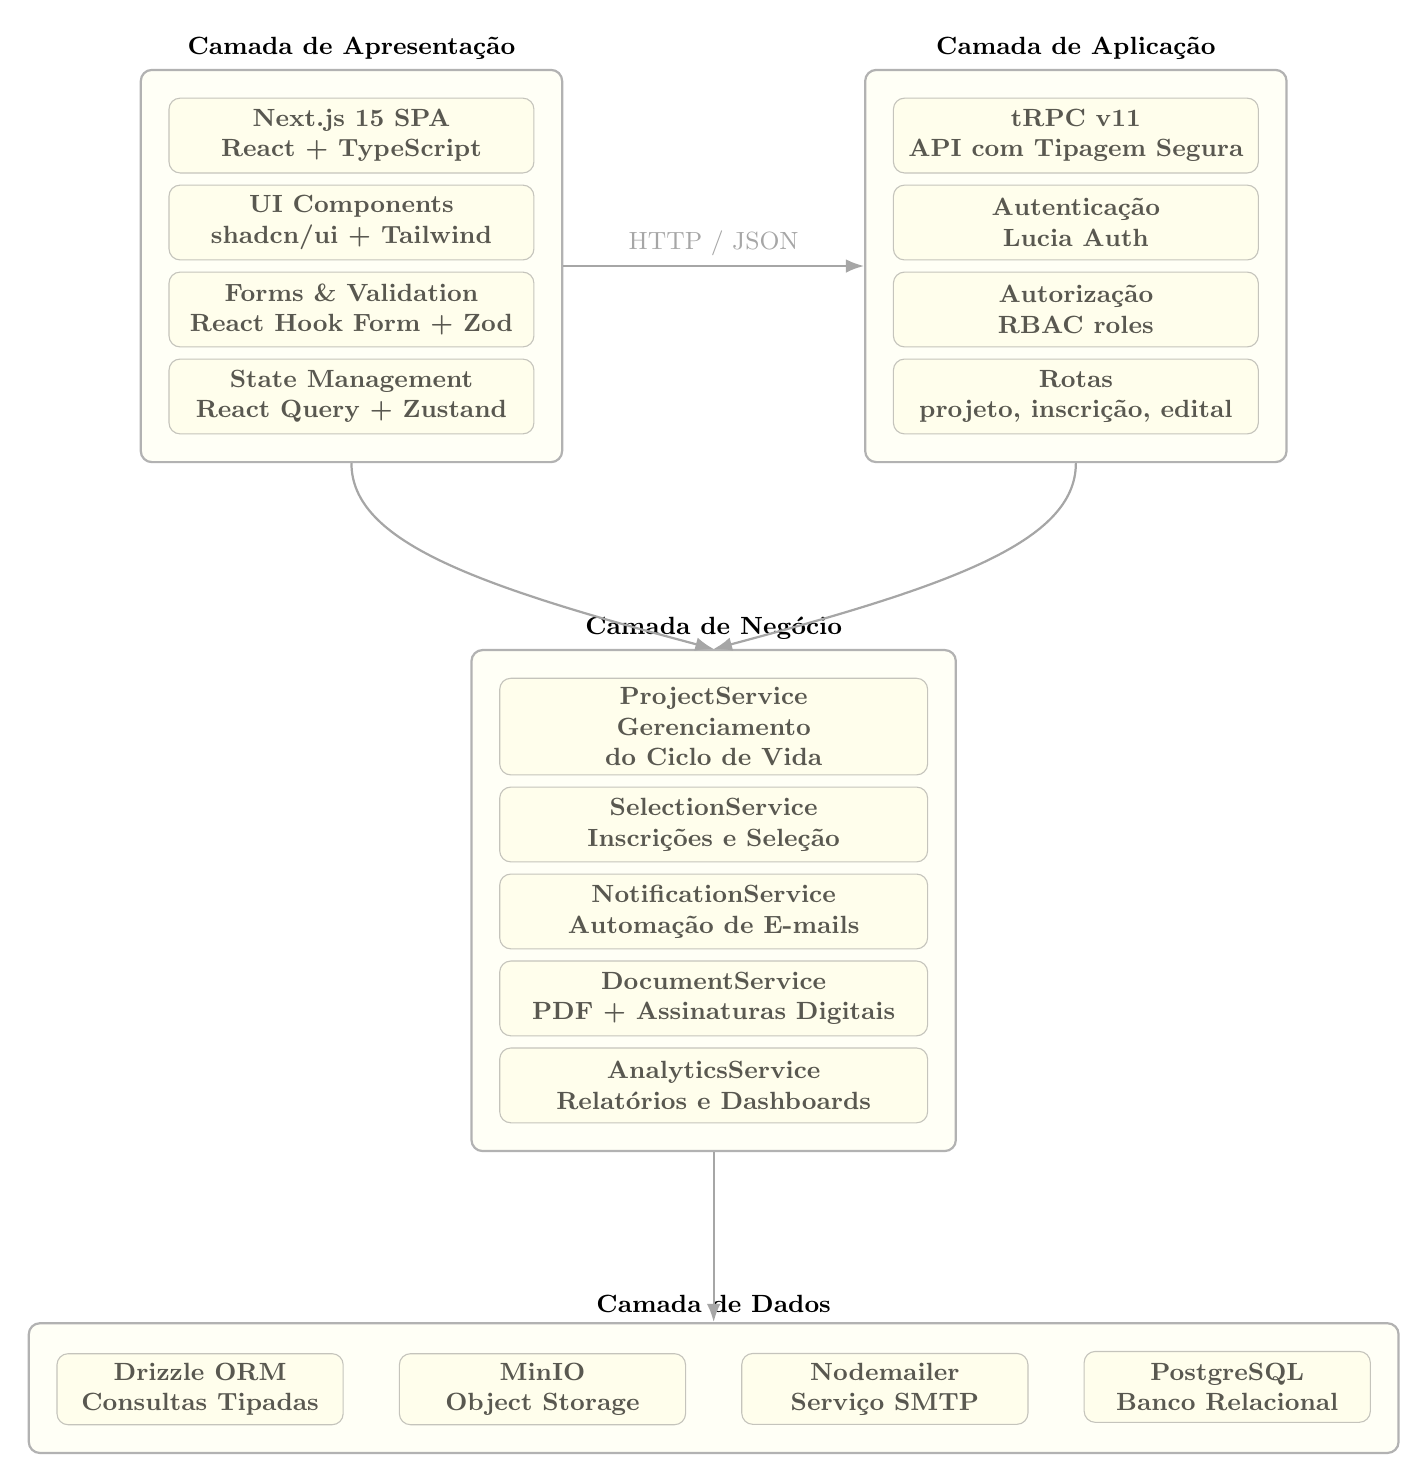
\begin{tikzpicture}[
    layer/.style={rounded corners, draw=gray!60, fill=yellow!10, fill opacity=0.35, draw opacity=1, thick, inner sep=10pt},
    box/.style={draw=gray!70, rounded corners, fill=yellow!6, text width=4.4cm, align=center, minimum height=0.95cm, font=\small\bfseries, text=black},
    smallbox/.style={draw=gray!70, rounded corners, fill=yellow!6, text width=5.2cm, align=center, minimum height=0.95cm, font=\small\bfseries, text=black},
    databox/.style={draw=gray!70, rounded corners, fill=yellow!6, text width=3.4cm, align=center, minimum height=0.9cm, font=\small\bfseries, text=black},
    connector/.style={-Latex, thick, gray!70}
  ]
    % Camada de Apresentação
    \matrix (presentation) [
      matrix of nodes,
      nodes={box},
      row sep=4pt,
      column sep=0pt,
      matrix anchor=north,
      anchor=north
    ] at (-4.6,0) {
      {Next.js 15 SPA\\React + TypeScript} \\
      {UI Components\\shadcn/ui + Tailwind} \\
      {Forms \& Validation\\React Hook Form + Zod} \\
      {State Management\\React Query + Zustand} \\
    };
    \node[layer, fit=(presentation-1-1)(presentation-4-1), label={[font=\small\bfseries]above:Camada de Apresentação}] (presentationLayer) {};

    % Camada de Aplicação
    \matrix (application) [
      matrix of nodes,
      nodes={box},
      row sep=4pt,
      column sep=0pt,
      matrix anchor=north,
      anchor=north
    ] at (4.6,0) {
      {tRPC v11\\API com Tipagem Segura} \\
      {Autenticação\\Lucia Auth} \\
      {Autorização\\RBAC roles} \\
      {Rotas\\projeto, inscrição, edital} \\
    };
    \node[layer, fit=(application-1-1)(application-4-1), label={[font=\small\bfseries]above:Camada de Aplicação}] (applicationLayer) {};

    % Camada de Negócio
    \coordinate (topMid) at ($(presentationLayer.south)!0.5!(applicationLayer.south)$);
    \matrix (business) [
      matrix of nodes,
      nodes={smallbox},
      row sep=4pt,
      column sep=0pt,
      matrix anchor=north,
      anchor=north
    ] at ($(topMid)+(0,-2.6)$) {
      {ProjectService\\Gerenciamento do Ciclo de Vida} \\
      {SelectionService\\Inscrições e Seleção} \\
      {NotificationService\\Automação de E-mails} \\
      {DocumentService\\PDF + Assinaturas Digitais} \\
      {AnalyticsService\\Relatórios e Dashboards} \\
    };
    \node[layer, fit=(business-1-1)(business-5-1), label={[font=\small\bfseries]above:Camada de Negócio}] (businessLayer) {};

    % Camada de Dados
    \matrix (data) [
      matrix of nodes,
      nodes={databox},
      row sep=0pt,
      column sep=0.7cm,
      matrix anchor=north,
      anchor=north
    ] at ($(businessLayer.south)+(0,-2.4)$) {
      {Drizzle ORM\\Consultas Tipadas} &
      {MinIO\\Object Storage} &
      {Nodemailer\\Serviço SMTP} &
      {PostgreSQL\\Banco Relacional} \\
    };
    \node[layer, fit=(data-1-1)(data-1-4), label={[font=\small\bfseries]above:Camada de Dados}] (dataLayer) {};

    % Conectores
    \draw[connector] (presentationLayer.east) -- node[above,font=\small]{HTTP / JSON} (applicationLayer.west);
    \draw[connector] (presentationLayer.south) .. controls +(0,-1.0) and +(-3,0.8) .. (businessLayer.north);
    \draw[connector] (applicationLayer.south) .. controls +(0,-1.0) and +(3,0.8) .. (businessLayer.north);
    \draw[connector] (businessLayer.south) -- (dataLayer.north);
  \end{tikzpicture}
  \caption{Arquitetura lógica do Sistema de Monitoria-IC.}
  \label{fig:architecture}
\end{figure}

\clearpage

\subsubsection{Camada de Apresentação}

Implementada como uma Single Page Application (SPA) usando Next.js 15, React e TypeScript, com interface responsiva construída a partir de componentes shadcn/ui e Tailwind CSS. O roteamento é dinâmico e protegido por papéis, o estado do cliente é coordenado por React Query e Zustand e os formulários utilizam React Hook Form com validações em Zod.

\subsubsection{Camada de Aplicação}

A camada de aplicação utiliza tRPC v11 para prover uma API \textit{type-safe} entre cliente e servidor. As procedures são organizadas por domínio (projeto, inscrição, edital, entre outros), com autenticação via Lucia Auth, validações automáticas com Zod e suporte a \textit{subscriptions} para atualizações em tempo quase real.

\subsubsection{Camada de Negócio}

A camada de negócio concentra serviços especializados: o \texttt{ProjectService} gerencia o ciclo de vida de projetos, o \texttt{SelectionService} processa inscrições e seleções, o \texttt{NotificationService} orquestra notificações por e-mail, o \texttt{DocumentService} cuida da geração de PDFs e das assinaturas e o \texttt{AnalyticsService} consolida dados para relatórios e painéis.

\subsubsection{Camada de Dados}

A camada de dados utiliza PostgreSQL com Drizzle ORM para persistência e MinIO para armazenamento de objetos. O esquema é relacional e normalizado, com integridade referencial e migrações versionadas e reversíveis; índices otimizam consultas frequentes, enquanto rotinas de backup e replicação asseguram resiliência.

\subsection{Modelo de Dados}

O modelo de dados foi projetado para capturar todas as entidades e relacionamentos do domínio de monitoria, seguindo princípios de normalização e integridade referencial. A Figura \ref{fig:data-model} apresenta as principais entidades e seus relacionamentos:

\clearpage

\begin{figure}[p]
  \centering
  \includegraphics[width=0.95\textwidth,keepaspectratio]{images/monitoria/data-model-new.png}
  \caption{Modelo de dados resumido do domínio de monitoria.}
  \label{fig:data-model}
\end{figure}

\clearpage

O dashboard administrativo consolida indicadores operacionais (projetos por status, períodos de inscrição, volume de candidaturas) e oferece navegação rápida para tarefas críticas do papel \textit{admin}, conforme a estrutura do menu lateral.

No núcleo de usuários, a entidade \texttt{user} concentra autenticação e perfil básico, estendida por perfis específicos de \texttt{professor} (dados acadêmicos) e \texttt{aluno} (matrícula, curso e CR), com papéis representados por \texttt{role} (\textit{admin}, \textit{professor}, \textit{student}). No eixo acadêmico, \texttt{departamento}, \texttt{curso}, \texttt{disciplina} e \texttt{periodo} descrevem a hierarquia institucional, os cursos vinculados, as disciplinas (com códigos e equivalências) e os semestres letivos. No domínio da monitoria, \texttt{projeto} evolui por estados bem definidos (DRAFT, SUBMITTED, APPROVED) e se relaciona a \texttt{projeto\_template} para reuso; \texttt{edital} organiza publicações por período; \texttt{inscricao} registra candidaturas e notas; \texttt{vaga} modela posições de monitor (BOLSISTA, VOLUNTARIO); e \texttt{documento} centraliza arquivos e assinaturas digitais.

\subsection{Fluxo de Processos}

O fluxo de monitoria é orquestrado em seis etapas contínuas que estruturam o semestre, conforme ilustrado na Figura \ref{fig:process-flow}. Na fase de planejamento e criação, a administração importa a planilha institucional de disciplinas e professores (SIAPE); o sistema identifica projetos individuais e coletivos, gera versões iniciais com base em templates de semestres anteriores e notifica docentes para revisão, edição e assinatura digital. Em seguida, ocorre a aprovação administrativa: projetos submetidos são avaliados com feedback, e a consolidação aprovada resulta em planilha com links em PDF encaminhada ao Instituto para viabilizar a solicitação de bolsas.

Com a definição do total de bolsas pela PROGRAD, inicia-se a alocação e a publicação do edital interno. O sistema impede excedentes na distribuição, permite que professores configurem vagas de voluntariado e conduz a geração do edital com assinatura digital do chefe de departamento, finalizando com publicação e notificações automáticas. A fase de inscrições e seleção disponibiliza um catálogo de vagas para os estudantes; o sistema captura automaticamente CR e notas (respeitando equivalências configuradas), enquanto os docentes avaliam candidatos e publicam resultados, contemplando bolsistas e voluntários.

Após a seleção, a etapa de aceite e consolidação final confirma as vagas: estudantes aceitam ou rejeitam convites, bolsistas informam dados bancários e a administração valida requisitos pendentes. O sistema produz a planilha final para a PROGRAD, encaminhada via Departamento. Por fim, o encerramento do ciclo envolve relatórios e certificados: os professores geram o relatório final da disciplina, os relatórios individuais dos monitores são assinados digitalmente (professor e aluno), a ata departamental é consolidada e são emitidos certificados para encaminhamento ao NUMOP, conforme detalhado na Figura \ref{fig:process-flow}.

\begin{figure}[H]
  \centering
  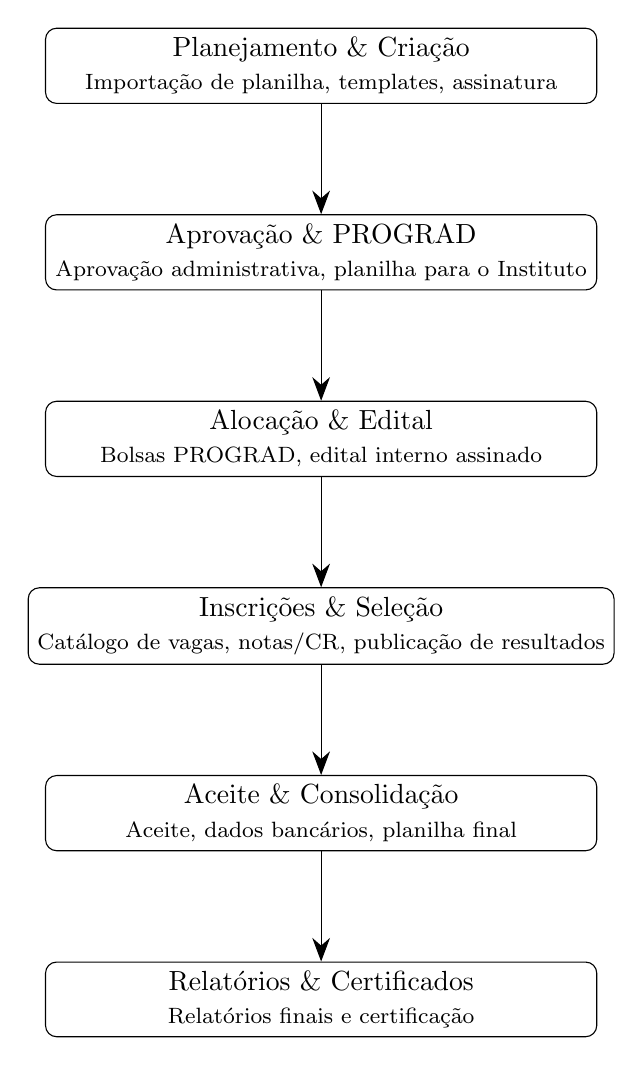
\begin{tikzpicture}[
    node distance=1.4cm,
    every node/.style={rounded corners, draw, align=center, minimum width=7cm, minimum height=0.9cm},
    >={Stealth[length=3mm]}
  ]
    \node (fase1) {Planejamento \& Criação\\\footnotesize Importação de planilha, templates, assinatura};
    \node[below=of fase1] (fase2) {Aprovação \& PROGRAD\\\footnotesize Aprovação administrativa, planilha para o Instituto};
    \node[below=of fase2] (fase3) {Alocação \& Edital\\\footnotesize Bolsas PROGRAD, edital interno assinado};
    \node[below=of fase3] (fase4) {Inscrições \& Seleção\\\footnotesize Catálogo de vagas, notas/CR, publicação de resultados};
    \node[below=of fase4] (fase5) {Aceite \& Consolidação\\\footnotesize Aceite, dados bancários, planilha final};
    \node[below=of fase5] (fase6) {Relatórios \& Certificados\\\footnotesize Relatórios finais e certificação};

    \draw[->] (fase1) -- (fase2);
    \draw[->] (fase2) -- (fase3);
    \draw[->] (fase3) -- (fase4);
    \draw[->] (fase4) -- (fase5);
    \draw[->] (fase5) -- (fase6);
  \end{tikzpicture}
  \caption{Fluxo de processos do semestre de monitoria.}
  \label{fig:process-flow}
\end{figure}

Em \textit{Gerenciar Projetos}, o administrador acompanha submissões, aprovações e gera a planilha consolidada para o Instituto/PROGRAD, garantindo padronização e trilhas de auditoria.

\subsection{Implementação e Tecnologias}

\subsubsection{Stack Tecnológico}

O sistema utiliza tecnologias modernas e consolidadas:

No \textit{frontend}, o sistema adota Next.js 15.1.4 (App Router) com TypeScript 5.x para \textit{type safety}. A interface utiliza Tailwind CSS e shadcn/ui; os formulários são implementados com React Hook Form e Zod; a sincronização de estado remoto e o cache são tratados por React Query. No \textit{backend}, a API \textit{type-safe} é construída com tRPC v11 e protegida por Lucia Auth; a persistência usa Drizzle ORM com PostgreSQL; documentos são armazenados no MinIO (S3-compatible) e o envio de e-mails é realizado via Nodemailer. Em \textit{DevOps}, a solução é containerizada com Docker e validada por uma pipeline no GitHub Actions que executa linting (Biome), verificação de tipos, testes unitários (Vitest), testes E2E (Playwright) e build de produção.

\subsubsection{Principais Routers tRPC}

O sistema organiza a lógica de negócio em routers especializados:

\begin{verbatim}
// src/server/api/root.ts
export const appRouter = createTRPCRouter({
  // Autenticação e usuários
  auth: authRouter,
  me: meRouter,
  user: userRouter,
  apiKey: apiKeyRouter,

  // Entidades acadêmicas
  departamento: departamentoRouter,
  curso: courseRouter,
  discipline: disciplineRouter,

  // Gestão de monitoria
  projeto: projetoRouter,
  projetoTemplates: projetoTemplatesRouter,
  edital: editalRouter,
  inscricao: inscricaoRouter,
  selecao: selecaoRouter,
  vagas: vagasRouter,

  // Administrativo
  importProjects: importProjectsRouter,
  scholarshipAllocation: scholarshipRouter,
  analytics: analyticsRouter,
  relatorios: relatoriosRouter,

  // Infraestrutura
  file: fileRouter,
  signature: signatureRouter,
  notificacoes: notificacoesRouter,
});
\end{verbatim}

\subsection{Interfaces do Sistema}

O sistema oferece interfaces especializadas para cada perfil de usuário, conforme exemplificado nas Figuras \ref{fig:landing} a \ref{fig:admin-departamentos}. A página inicial (Figura \ref{fig:landing}) apresenta a proposta do sistema, acesso ao login institucional e comunicação de períodos de inscrição quando ativos, funcionando como ponto de entrada para estudantes, professores e administradores. A tela de login (Figura \ref{fig:login}) valida credenciais locais ou redireciona ao CAS quando habilitado, estabelecendo a sessão do usuário e direcionando ao dashboard apropriado.

\begin{figure}[h!]
  \centering
  \includegraphics[width=\linewidth]{images/monitoria/landing.png}
  \caption{Página inicial pública do sistema.}
  \label{fig:landing}
\end{figure}

\begin{figure}[h!]
  \centering
  \includegraphics[width=\linewidth]{images/monitoria/login.png}
  \caption{Tela de login local do sistema.}
  \label{fig:login}
\end{figure}

O dashboard administrativo (Figura \ref{fig:dashboard}) consolida indicadores operacionais (projetos por status, períodos de inscrição, volume de candidaturas) e oferece navegação rápida para tarefas críticas do papel \textit{admin}. A interface de assinatura de projetos (Figura \ref{fig:professor-assinatura}) permite que o professor visualize o PDF gerado, use a assinatura padrão do perfil ou desenhe uma nova assinatura antes de submeter para análise administrativa.

\begin{figure}[h!]
  \centering
  \includegraphics[width=\linewidth]{images/monitoria/admin-dashboard.png}
  \caption{Dashboard administrativo com métricas.}
  \label{fig:dashboard}
\end{figure}

\begin{figure}[h!]
  \centering
  \includegraphics[width=\linewidth]{images/monitoria/professor-assinatura-documentos.png}
  \caption{Assinatura de projeto pelo professor.}
  \label{fig:professor-assinatura}
\end{figure}

Para estudantes, a tela de inscrição (Figura \ref{fig:student-inscricao}) oferece filtros por departamento e tipo de vaga, busca por título/professor e exibe avisos sobre o período ativo; quando o período está fechado, os componentes permanecem acessíveis para consulta e planejamento. A tela de resultados (Figura \ref{fig:student-resultados}) permite que o aluno acompanhe o status de cada inscrição (selecionado bolsista/voluntário, lista de espera, não selecionado) e o resumo agregado por categoria.

\begin{figure}[h!]
  \centering
  \includegraphics[width=\linewidth]{images/monitoria/student-inscricao-monitoria.png}
  \caption{Inscrição do aluno em projetos de monitoria.}
  \label{fig:student-inscricao}
\end{figure}

\begin{figure}[h!]
  \centering
  \includegraphics[width=\linewidth]{images/monitoria/student-resultados.png}
  \caption{Resultados das seleções para o aluno.}
  \label{fig:student-resultados}
\end{figure}

As funcionalidades administrativas incluem o gerenciamento de projetos (Figura \ref{fig:projetos}), onde o administrador acompanha submissões e aprovações e gera a planilha consolidada para o Instituto/PROGRAD; a gestão de editais (Figura \ref{fig:editais}), que permite configurar datas, pontos de prova e bibliografia, solicitar assinatura digital do chefe do departamento e publicar com notificações automáticas; e a alocação de bolsas (Figura \ref{fig:bolsas}), que impede excedentes em relação ao total de bolsas concedidas pela PROGRAD.

\begin{figure}[h!]
  \centering
  \includegraphics[width=\linewidth]{images/monitoria/admin-manage-projects.png}
  \caption{Gerenciamento de projetos por semestre.}
  \label{fig:projetos}
\end{figure}

\begin{figure}[h!]
  \centering
  \includegraphics[width=\linewidth]{images/monitoria/admin-edital-management.png}
  \caption{Gestão de editais com status e ações.}
  \label{fig:editais}
\end{figure}

\begin{figure}[h!]
  \centering
  \includegraphics[width=\linewidth]{images/monitoria/admin-scholarship-allocation.png}
  \caption{Interface de alocação de bolsas.}
  \label{fig:bolsas}
\end{figure}

Completam as interfaces administrativas a gestão de usuários (Figura \ref{fig:admin-users}), onde a administração pesquisa, filtra e gerencia contas mantendo coerência com regras institucionais; o gerenciamento de arquivos (Figura \ref{fig:admin-files}), que centraliza documentos com versionamento e metadados para auditoria; e a importação de planejamento (Figura \ref{fig:admin-import}), que processa planilhas do planejamento e emite relatório de inconsistências. As telas de cursos (Figura \ref{fig:admin-cursos}) e departamentos (Figura \ref{fig:admin-departamentos}) permitem manter a estrutura acadêmica essencial para vínculos de disciplinas e projetos.

\begin{figure}[h!]
  \centering
  \includegraphics[width=\linewidth]{images/monitoria/admin-users.png}
  \caption{Administração de usuários.}
  \label{fig:admin-users}
\end{figure}

\begin{figure}[h!]
  \centering
  \includegraphics[width=\linewidth]{images/monitoria/admin-files.png}
  \caption{Gerenciamento de arquivos.}
  \label{fig:admin-files}
\end{figure}

\begin{figure}[h!]
  \centering
  \includegraphics[width=\linewidth]{images/monitoria/admin-import-projects.png}
  \caption{Importação de planejamento.}
  \label{fig:admin-import}
\end{figure}

\begin{figure}[h!]
  \centering
  \includegraphics[width=\linewidth]{images/monitoria/admin-cursos.png}
  \caption{Gestão de cursos.}
  \label{fig:admin-cursos}
\end{figure}

\begin{figure}[h!]
  \centering
  \includegraphics[width=\linewidth]{images/monitoria/admin-departamentos.png}
  \caption{Gestão de departamentos.}
  \label{fig:admin-departamentos}
\end{figure}

\section{Avaliação Experimental}
\label{sec:evaluation}

O objetivo desta avaliação experimental é validar a efetividade do Sistema de Monitoria-IC em dois eixos fundamentais: (i) \textbf{eficiência operacional}, mensurando ganhos quantitativos em tempo, redução de erros e automação de tarefas em relação ao processo manual anterior; e (ii) \textbf{usabilidade e satisfação}, coletando percepções de usuários reais (professores, administradores e estudantes) quanto à facilidade de uso, transparência e impacto no cotidiano acadêmico. A avaliação busca demonstrar que a solução proposta não apenas funciona tecnicamente, mas efetivamente melhora o processo de gestão de monitoria na prática institucional.

\subsection{Metodologia}

O desenho de avaliação contempla: (i) \textit{logs} de aplicação (latência, throughput e erros), (ii) extração de métricas operacionais (tempo de ciclo por etapa, volume de inscrições e seleções, tempo de publicação de resultados), (iii) questionários estruturados para docentes, discentes e administradores após execução completa do fluxo de monitoria com o sistema e (iv) comparação histórica com semestres anteriores (baseline manual) conforme as fases descritas em \S\ref{sec:system}. Para validar a usabilidade, foi definida uma avaliação com atores reais que executam o processo completo desde criação de projeto até aceite de vaga, respondendo questionários estruturados ao final.

\medskip

\subsection{Resultados}

\begin{figure}[h!]
  \centering
  \includegraphics[width=0.4\linewidth]{images/TODO.jpeg}
  \caption{Resultados quantitativos pendentes de coleta e análise.}
  \label{fig:todo-resultados}
\end{figure}

\FloatBarrier

\section{Conclusão e Trabalhos Futuros}
\label{sec:conclusion}

Este trabalho apresentou o desenvolvimento do Sistema de Monitoria-IC como solução específica para o \textit{workflow} completo de monitoria. As contribuições centrais abrangem a automação integral de processos (da importação de dados à emissão de certificados), a adoção de uma arquitetura moderna e escalável que separa SPT e funcionalidades gerenciais e a disponibilização de uma base estruturada que viabiliza futuras pesquisas e implantações em ambiente institucional.

A adoção plena do sistema tem o potencial de produzir efeitos mensuráveis no cotidiano administrativo, reduzindo o tempo gasto em tarefas repetitivas, eliminando retrabalho e padronizando procedimentos entre departamentos. Na dimensão estratégica, a consolidação de dados permite análises históricas e de tendências, qualificando a tomada de decisão e abrindo espaço para políticas institucionais orientadas por evidências. Do ponto de vista pedagógico, a maior facilidade de participação tende a ampliar o alcance do programa, a transparência reforça a confiança de todos os atores e a economia de tempo contribui para liberar docentes para atividades-fim.

Apesar dos resultados positivos, permanecem desafios: a integração com o sistema acadêmico ainda é parcial para captura automática de CR e histórico; o escopo atual está restrito ao Instituto de Computação, exigindo adaptações para expansão; parte do fluxo depende de setores externos (PROGRAD, NUMOP), o que mantém etapas manuais; e a ausência de um aplicativo móvel nativo pode limitar o acesso em determinados contextos.

O plano de evolução contempla três horizontes. No curto prazo (seis meses), prioriza-se a conclusão da integração com o sistema acadêmico (SIAC), a entrega do módulo de certificados digitais, o desenvolvimento do aplicativo móvel (React Native) e a expansão controlada para outros departamentos da UFBA. No médio prazo (cerca de um ano), o foco recai sobre um sistema de recomendação para \textit{matching} aluno–projeto, analytics avançado com \textit{machine learning}, integrações com plataformas de ensino (como Moodle) e a disponibilização de uma API pública para sistemas terceiros. No longo prazo, busca-se generalizar o uso para outras universidades, criar um marketplace de templates entre instituições, conduzir estudos longitudinais sobre o impacto da monitoria e publicar o projeto como software livre para a comunidade acadêmica.

O Sistema de Monitoria-IC representa um avanço significativo na modernização da gestão acadêmica universitária. Ao digitalizar e automatizar processos tradicionalmente manuais, o sistema não apenas aumenta a eficiência operacional, mas também estabelece uma base sólida para a transformação digital contínua das universidades brasileiras. A experiência de desenvolvimento e implantação deste sistema demonstra que é possível criar soluções tecnológicas específicas para problemas acadêmicos complexos, utilizando tecnologias modernas e práticas de engenharia de software consolidadas. O sucesso inicial na UFBA sugere alto potencial de replicação em outras instituições que enfrentam desafios similares. Esperamos que este trabalho inspire outras iniciativas de modernização administrativa no ambiente universitário e contribua para o avanço da discussão sobre transformação digital na educação superior brasileira. O código fonte e documentação estarão disponíveis publicamente após a conclusão das funcionalidades principais, permitindo que outras instituições adaptem e evoluam a solução conforme suas necessidades específicas.

\FloatBarrier

\section*{Agradecimentos}

Agradecemos ao Instituto de Computação da UFBA pelo apoio institucional, aos professores e alunos que participaram dos testes piloto, e à equipe de TI que viabilizou a infraestrutura necessária.

\bibliographystyle{apalike-sol}
\bibliography{references}

\end{document}